\chapter{Testy}

\paragraph{}
V predošlej kapitole sme bližšie popísali implementáciu našich algoritmov. Táto kapitola sa zameriava na evalváciu výsledkov z týchto algoritmov. Keďže celá táto práca sa zaoberá implementáciou algoritmov na generovanie hesiel pomocou vstupného slovníka, bolo potrebné si nájsť vhodný vstupný slovník. Podarilo sa nám nájsť online zdroj slovníkov \cite{dictionaries}, ktorý obsahuje slovníky s usporiadanými heslami podľa pravdepodobnosti výskytu. Slovník je formátovaný v dvoch stĺpcoch, kde prvý obsahuje informáciu o počte výskytov daného heslá a druhý je samotné heslo.

\section{Časová náročnosť}
V tomto základnom teste sme spustili naše algoritmy a počítali čas behu algoritmov pre jednotlivé parametre spustenia. Pre všetky testy používame slovník \emph{phpbb} stiahnutý z \cite{dictionaries}. Slovník sme upravovali aby obsahoval len heslá zodpovedajúce maximálnej dĺžke hesiel, ktoré generuje bezkontextová gramatika. Týmto sme znížili pravdepodobnosť Markovského zdroja generovať heslá dlhšie ako stanovené maximum pre gramatiku. Stĺpec \emph{d} označuje maximálnu dĺžku generovaných hesiel zatiaľ čo stĺpec \emph{p} vyjadruje maximálnu veľkosť jednoduchého neterminálu respektíve dĺžku prefixu podľa ktorého sa rozhoduje Markovský zdroj. Tieto časové testy boli spúšťané na procesore Intel® Core™ i5-4690K s rýchlosťou 3.50GHz na operačnom systéme Windows 10. Namerané hodnoty zobrazené v tabuľke sú uvedené v sekundách.

\begin{table}[]
\centering
\caption{Časy pre slovník phpbb}
\label{tphpbb}
\begin{tabular}{lll|lllllll}
       & d & p & GEN     & 10000  & 50000  & 100000 & 500000 & 1000000 & 5000000 \\ \hline
CFG    & 6 & 2 & 0.103   & 0.754  & 3.504  & 7.097  & 35.109 & 71.129  & 369.057 \\
CFG    & 6 & 3 & 0.32    & 2.696  & 5.441  & 9.028  & 37.121 & 72.181  & 354.763 \\
CFG    & 6 & 4 & 6.053   & 2.621  & 5.53   & 8.96   & 37.515 & 73.744  & 367.655 \\
CFG    & 6 & 5 & 156.141 & 47.595 & 50.767 & 54.054 & 81.957 & 116.699 & 397.522 \\
Markov & 6 & 2 & ---     & 1.284  & 3.936  & 7.469  & 34.533 & 68.029  & 337.949 \\
Markov & 6 & 3 & ---     & 2.218  & 4.839  & 8.28   & 35.406 & 69.88   & 347.756 \\
Markov & 6 & 4 & ---     & 4.833  & 7.926  & 10.874 & 38.463 & 81.074  & 373.771 \\ \hline
       & d & p & GEN     & 10000  & 50000  & 100000 & 500000 & 1000000 & 5000000 \\ \hline
CFG    & 7 & 2 & 0.21    & 0.808  & 3.646  & 7.011  & 35.11  & 70.911  & 361.186 \\
CFG    & 7 & 3 & 0.419   & 0.84   & 3.607  & 7.156  & 36.138 & 71.242  & 361.462 \\
CFG    & 7 & 4 & 6.182   & 3.022  & 5.459  & 9.041  & 37.589 & 73.397  & 364.075 \\
CFG    & 7 & 5 & 158.024 & 53.649 & 52.981 & 56.456 & 84.178 & 119.034 & 402.945 \\
Markov & 7 & 2 & ---     & 1.648  & 4.361  & 7.753  & 34.48  & 68.228  & 349.683 \\
Markov & 7 & 3 & ---     & 2.864  & 5.575  & 9.602  & 37.016 & 71.108  & 346.98  \\
Markov & 7 & 4 & ---     & 8.19   & 10.772 & 13.921 & 43.673 & 79.005  & 379.443 \\ \hline
       & d & p & GEN     & 10000  & 50000  & 100000 & 500000 & 1000000 & 5000000 \\ \hline
CFG    & 8 & 2 & 0.588   & 0.905  & 3.662  & 7.094  & 36.179 & 71.394  & 369.456 \\
CFG    & 8 & 3 & 0.818   & 0.939  & 3.71   & 7.338  & 36.871 & 74.814  & 362.259 \\
CFG    & 8 & 4 & 6.758   & 3.015  & 5.182  & 8.512  & 34.945 & 68.242  & 335.426 \\
CFG    & 8 & 5 & 159.983 & 51.749 & 49.595 & 53.055 & 78.314 & 110.507 & 374.249 \\
Markov & 8 & 2 & ---     & 2.462  & 5.029  & 8.441  & 34.9   & 68.778  & 337.725 \\
Markov & 8 & 3 & ---     & 4.679  & 7.333  & 10.563 & 38.329 & 71.626  & 345.412 \\
Markov & 8 & 4 & ---     & 12.857 & 16.485 & 24.572 & 54.914 & 87.455  & 428.908
\end{tabular}
\end{table}

\paragraph{}


\section{Výstupné heslá}
Po overení časovej zložitosti generovania hesiel pomocou jednotlivých algoritmov sme na výsledné heslá aplikovali viaceré metriky. Cieľom týchto testov bolo ukázať výhody a slabiny jednotlivých algoritmov a spraviť ich vzájomne porovnanie v zmysle šancí na nájdenie hľadaného heslá. Vzhľadom na to, že v praxi sa trendy medzi používanými heslami môžu meniť a časom by mohla drvivá väčšina ľudí používať bezpečné heslá, tieto metriky nie sú záväzne a nevypovedajú o tom ako sa budú jednotlivé algoritmy správať ak by boli použité v praxi.

\subsection{Heslá zo slovníka}
Ako prvú metriku sme skúmali koľko hesiel zo slovníka gramatika vygenerovala po vygenerovaní určitého počtu hesiel. Na grafoch, ktoré boli výstupom tohto testu sme na vodorovnej osi znázornili počet hesiel vygenerovaných gramatikou zatiaľ čo na vertikálnej osi je počet hesiel slovníka, ktoré sa medzi nimi nachádzajú. Pri tomto teste sme nechali oba algoritmy generovať 100 miliónov hesiel k čomu bol použitý slovník obsahujúci 13 331 008 rôznych hesiel dĺžky 12 a menej znakov.

\paragraph{}
Nižšie vidíme grafy znázorňujúce vývoj počtu vygenerovaných hesiel, ktoré sa nachádzajú v slovníku. Prvý graf popisuje priebeh trendu v pohľade na všetky vygenerované heslá. Vidíme, že počet hesiel zo slovníka lineárne stúpa s počtom vygenerovaných hesiel. Vidíme, že zo 100 miliónov vygenerovaných je takmer polovica zložená z hesiel, ktoré sa nachádzajú v slovníku. Toto číslo je trojnásobok všetkých hesiel slovníka, toto je spôsobené tým, že Markov zdroj nekontroluje, ktoré heslá už boli vygenerované a veľké množstvo ich opakuje.

\begin{figure}[h]
    \centering
    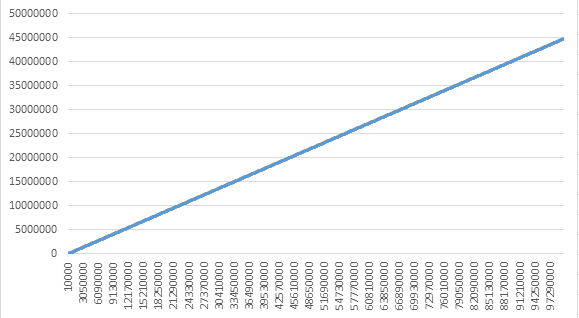
\includegraphics[width=1\textwidth]{Accuracy_mark}
    \caption{Počet vygenerovaných hesiel zo slovníka - Markovský zdroj}
    \label{fig:AccMark}
\end{figure}
\paragraph{}
Tento algoritmus vygeneroval len niečo málo cez 42 miliónov unikátnych hesiel. Z týchto unikátnych hesiel sa približne 2,5 milióna nachádza vo vstupnom slovníku. Z týchto grafov môžme vidieť, že Markov zdroj má problém so zbytočným generovaním veľkého množstva hesiel duplicitne. Naopak je vidieť, že učiaci algoritmus založený na prefixoch o veľkosti \emph{k} je efektívny čo sa týka napodobenia pravdepodobností, ktoré dostal na vstupe.

\begin{figure}[h]
    \centering
    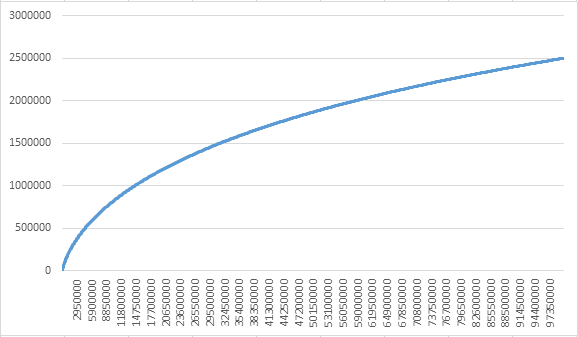
\includegraphics[width=1\textwidth]{Accuracy_mark_uniq}
    \caption{Počet vygenerovaných hesiel zo slovníka - Markovský zdroj - Unikátne}
    \label{fig:AccMarkUniq}
\end{figure}

\paragraph{}
Na \ref{fig:AccCFG} vidíme priebeh hodnôt pre nami definované a implementované riešenie pomocou bezkontextových gramatík. Toto riešenie má na rozdiel od Markovho zdroja omnoho pomalší rast počtu hesiel patriacich do slovníka. Pri 100 miliónoch generovaných hesiel to je niečo málo pod 700 tisíc. Dôvod pre takéto relatívne malé percento vygenerovaných hesiel zo slovníka môže byť práve vlastnosť gramatiky učiť sa vzory hesiel. Keďže vo vstupnom slovníku existovalo málo hesiel, ktoré mali obrovský počet výskytov, gramatika sa zamerala na generovanie hesiel s veľmi podobným vzorom.

\begin{figure}[h]
    \centering
    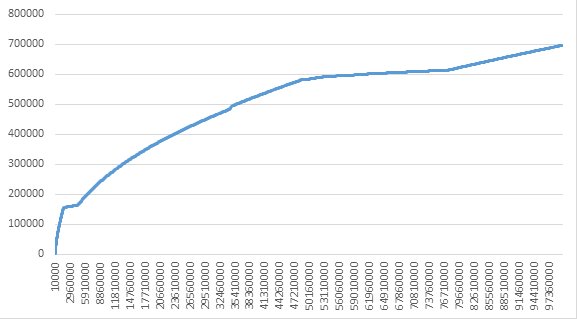
\includegraphics[width=1\textwidth]{Accuracy_CFG}
    \caption{Počet vygenerovaných hesiel zo slovníka - Gramatika}
    \label{fig:AccCFG}
\end{figure}

Ďalej sme taktiež skúmali ako sa správajú nami implementované algoritmy ma menších dátach. Na obrázku \ref{fig:Acc6} je znázornený graf priebehu generovania hesiel, ktoré sa nachádzajú vo vstupnom slovníku. Na vodorovnej osi je ukázaný počet vygenerovaných hesiel, v tomto prípade to bolo 5 miliónov hesiel. Výška čiar určuje množstvo hesiel, ktoré boli nájdene vo vstupnom slovníku. Pre Markovské zdroje sa toto číslo počíta z počtu unikátnych hesiel, ktoré boli vygenerované. Všimli sme si, že priebehy jednotlivých algoritmov sa náramne podobajú logaritmickej krivke. Taktiež si môžme všimnúť, že algoritmus používajúci Markovské zdroje je v tejto metriky opäť lepší ako algoritmus používajúci pravdepodobnostné bezkontextové gramatiky. Použili sme slovník phpbb stiahnutý z \cite{dictionaries}, ktorý sme upravili aby všetky heslá mali dĺžku najviac 6 znakov. Takto upravený slovník mal nakoniec 55 744 rôznych hesiel.

\begin{figure}[h]
    \centering
    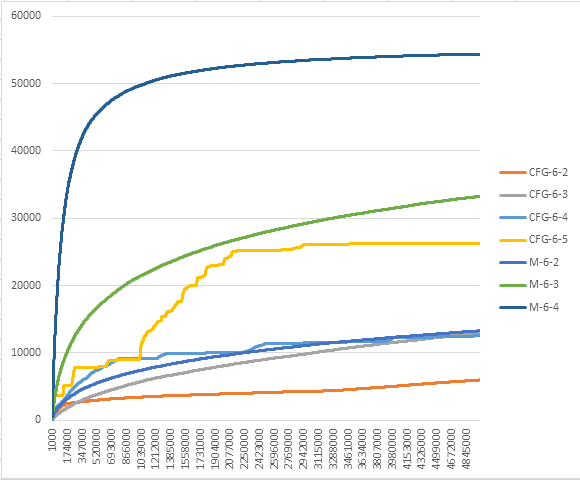
\includegraphics[width=1\textwidth]{Accuracy_6}
    \caption{Počet vygenerovaných hesiel zo slovníka - dĺžka 6}
    \label{fig:Acc6}
\end{figure}

Po zhliadnutí rovnakého grafu pre algoritmy pustené pre generovanie hesiel dĺžky 7 a s upraveným slovníkom phpbb obsahujúcim heslá najviac dĺžky 7 sme si všimli, že množstvo hesiel zo vstupného slovníka generovaných našimi algoritmami sa nezmenilo až na Markovské zdroje s prefixom 4. V tomto teste bola veľkosť vstupného slovníka 88 416 hesiel.

\begin{figure}[h]
    \centering
    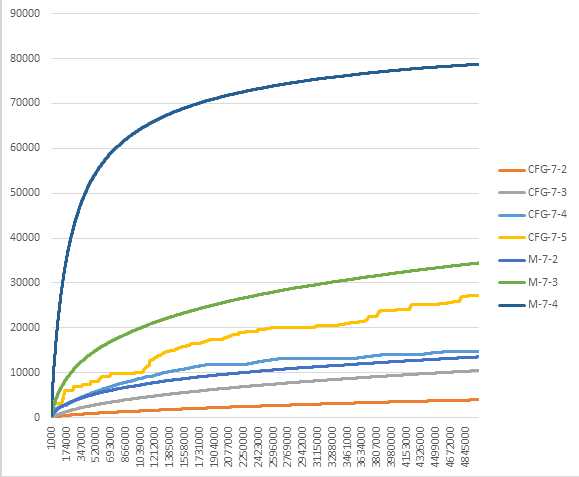
\includegraphics[width=1\textwidth]{Accuracy_7}
    \caption{Počet vygenerovaných hesiel zo slovníka - dĺžka 7}
    \label{fig:Acc7}
\end{figure}

Nakoniec sme tento istý test opäť spustili na všetkých algoritmoch. Tentokrát vstupné parametre a slovník boli nastavené na generovanie hesiel maximálnej dĺžky 8. Takto upravený slonvík phpbb obsahoval 143 675 hesiel z ktorých až 100 tisíc bolo vygenerovaných algoritmom používajúcim Markovské zdroje s prefixom nastaveným na dĺžku 4. Avšak taktiež ako pri dĺžke 7, ostatné inštancie algoritmov nepresiahli ani 40 tisíc vygenerovaných hesiel.

\begin{figure}[h]
    \centering
    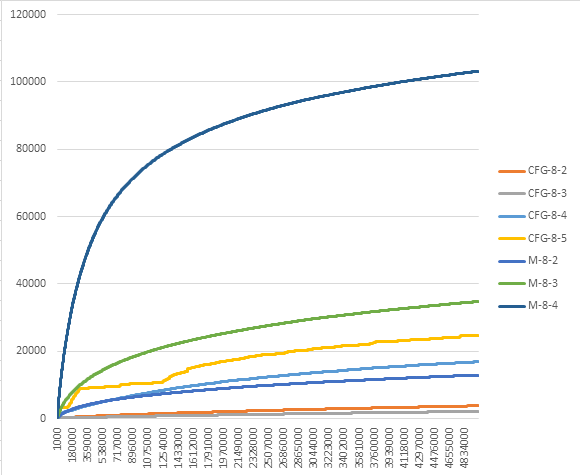
\includegraphics[width=1\textwidth]{Accuracy_8}
    \caption{Počet vygenerovaných hesiel zo slovníka - dĺžka 8}
    \label{fig:Acc8}
\end{figure}

\paragraph{}
Na základe \ref{fig:AccMarkUniq} a \ref{fig:AccCFG} vidíme, že nami navrhnutá metóda pomocou bezkontextových gramatík síce negeneruje veľa hesiel zo vstupného slovníka počas prvých miliónov vygenerovaných hesiel. Tento problém by sa dal vyriešiť, tým že by sme vždy ako prvé na výstup poslali všetky heslá zo slovníka, keďže ten býva zanedbateľne malý oproti veľkosti priestoru hesiel, ktorý musíme prehľadať aby sme definitívne našli hľadané heslo. Pri analyzovaní týchto dát nemôžme zabudnúť, že terajšia verzia algoritmu používajúceho Markovský zdroj negeneruje celý priestor hesiel určenej dĺžky.

\subsection{Miery presnosti}
Pod týmto pojmom rozumieme metriky popisujúce nielen kvantitu nami generovaných hesiel patriacich do slovníka, ale snažia sa bližšie vyhodnotiť ako rýchlo sa gramatika dostane k heslám, ktoré boli podľa vstupného slovníka označené za najpravdepodobnejšieho.

\paragraph{}
Stĺpce tabuľky \ref{mieryPresnosti} vyjadrujú hodnoty jednotlivých metrík pre daný algoritmus.
\begin{itemize}
	\item \emph{PPS} - Priemerná Pozícia v Slovníku - Vyjadruje priemernú pozíciu vo vstupnom slovníku hesiel, ktoré boli vygenerované algoritmom na výstupe
	\item \emph{PPS \%} - Priemerná Pozícia v Slovníku - Vyjadruje percentuálnu pozíciu vrámci slovníku hesiel, ktoré boli vygenerované algoritmom na výstupe
	\item \emph{RPSV} - Rozdiel Pozície v Slovníku a na Výstupe - Rozdiel v pozícií na vstupe a na výstupe algoritmu prenásobený percentuálnym počtom výskytov vo vstupnom slovníku
\end{itemize}

\[ \frac{\displaystyle\sum_{i=1}^{k}((indG_i - indS_x) * \frac{v_{ind_x}}{\sum_{j=1}^{n}v_j})}{k} \]

Vzorec vyjadrujúci mieru RPSV, kde \emph{n} vyjadruje počet hesiel vo vstupnom slovníku a \emph{k} je počet výskytov hesiel zo vstupného slovníka medzi generovanými. Hodnota \emph{\(indG_i\)} určuje poradie i-tého heslá nachádzajúceho sa vo vstupnom aj výstupnom slovníku vrámci generovaného slovníka. Hodnota \emph{\(indS_i\)} vyjadruje tú istú hodnotu pre vstupný slovník. Hodnoty \emph{\(v_i\)} sú počty výskytov hesiel zadefinované vo vstupnom slovníku.

\paragraph{}
Priemerná pozícia v slovníku ukazuje ako pravdepodobné heslá v priemernom prípade generuje náš algoritmus. Keďže toto číslo sa často krát zdá veľké, prikladáme k nemu v druhom stĺpci jeho percentuálnu hodnotu. Hodnoty d a p vyjadrujú maximálnu dĺžku hesiel v slovníku a dĺžku použitých prefixov v Markovskom zdroji. Pre hodnoty 6,7,8 parametru \emph{d} sme použili slovník \emph{phppbb} upravený na heslá relevantnej dĺžky. Pre hodnoty \emph{d} rovné 12 sme použili omnoho robustnejší slovník \emph{rockyou}, skladajúci sa z takmer 14 miliónov unikátnych hesiel.

\begin{table}[]
\centering
\caption{Miery presnosti}
\label{mieryPresnosti}
\begin{tabular}{lll|lll}
       & d  & p & PPS & PPS \% & RPSV \\ \hline
CFG    & 6  & 2 & 31328    & 56.199       & 36.567     \\
CFG    & 6  & 3 & 26358    & 47.285       & 37.749     \\
CFG    & 6  & 4 & 31033    & 55.670       & 19.673     \\
CFG    & 6  & 5 & 28554    & 51.224       & 21.397     \\
CFG    & 7  & 2 & 47454    & 53.672       & 26.489     \\
CFG    & 7  & 3 & 40343    & 45.629       & 25.831     \\
CFG    & 7  & 4 & 46739    & 52.863       & 16.648     \\
CFG    & 7  & 5 & 46718    & 52.840       & 21.715     \\
CFG    & 8  & 2 & 88521    & 61.612       & 16.139     \\
CFG    & 8  & 3 & 61113    & 42.536       & 22.384     \\
CFG    & 8  & 4 & 70500    & 49.069       & 15.028     \\
CFG    & 8  & 5 & 75570    & 52.598       & 14.749     \\
Markov & 6  & 2 & 25219    & 45.241       & 28.307     \\
Markov & 6  & 3 & 25959    & 46.568       & 14.815     \\
Markov & 6  & 4 & 27705    & 49.701       & 3.649     \\
Markov & 7  & 2 & 39090    & 44.212       & 21.289     \\
Markov & 7  & 3 & 40283    & 45.561       & 13.321     \\
Markov & 7  & 4 & 43232    & 48.896       & 4.700     \\
Markov & 8  & 2 & 61688    & 42.936       & 15.745     \\
Markov & 8  & 3 & 66401    & 46.216       & 9.701     \\
Markov & 8  & 4 & 68291    & 47.532       & 4.596     \\ \hline \hline
CFG    & 12 & 4 & 3781788    & 28.3       & 5.879     \\
Markov & 12 & 4 & 4609712    & 34.5       & 2.191    
\end{tabular}
\end{table}

\paragraph{}
Z tabuľky \ref{mieryPresnosti} môžme vidieť že obom našim algoritmom prospieva navýšenie vstupnej informácie o heslách. Toto je vidieť na jak na percentuálnych hodnotách priemernej pozície v slovníku tak aj na rozdieloch pozícií medzi vstupným a vygenerovaným slovníkom. Hodnota rozdielov pozícií má vyjadrovať presnosť generovania hesiel v správnom poradí, alebo v poradí blízkom tomu zo vstupného slovníka.